\documentclass[tikz,border=5pt]{standalone}
\usepackage{fontspec}
\usetikzlibrary{arrows.meta,positioning,calc}
\setmainfont{TeX Gyre Heros}
\definecolor{ink}{HTML}{24364B}
\definecolor{blue}{HTML}{2878B5}
\definecolor{orange}{HTML}{D86613}
\definecolor{green}{HTML}{15956F}
\definecolor{violet}{HTML}{8464B8}
\definecolor{band}{HTML}{E8EEF4}
\definecolor{muted}{HTML}{66788A}
\begin{document}
\special{pdf:minorversion 5}
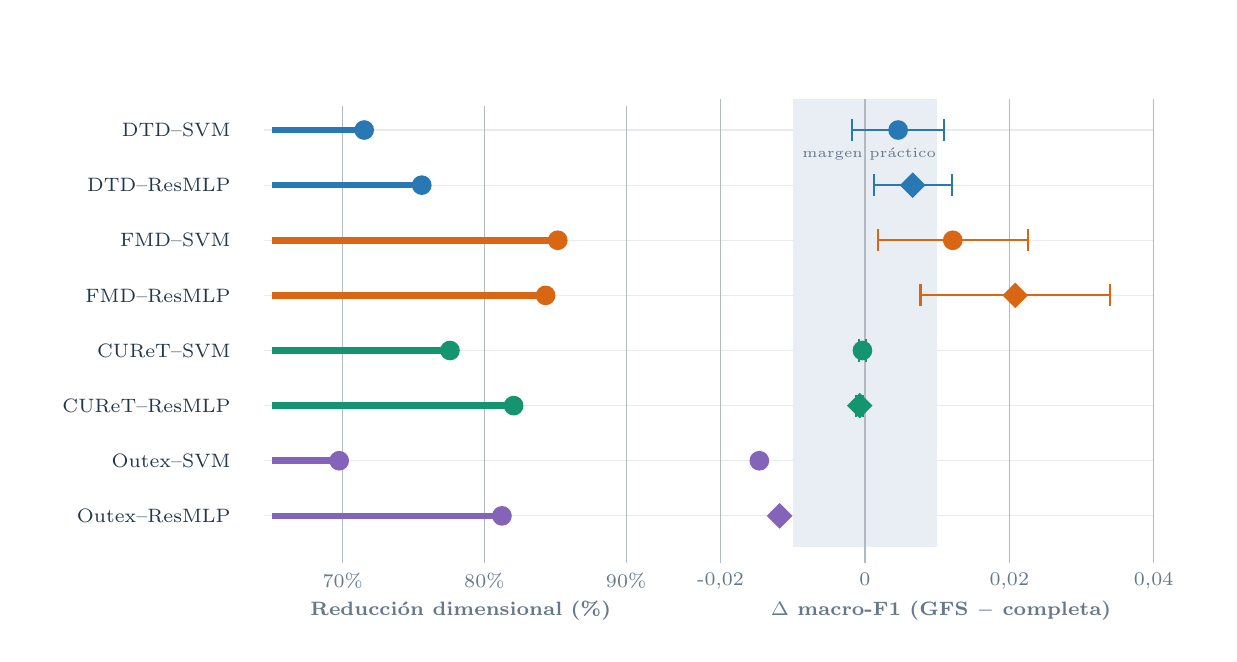
\begin{tikzpicture}[x=1mm,y=1mm,font=\small]
  \path[use as bounding box] (0,-8) rectangle (150,69);
  % Shared rows; left panel encodes compression, right panel paired performance.
  \foreach \label/\yy in {DTD--SVM/56,DTD--ResMLP/49,FMD--SVM/42,FMD--ResMLP/35,CUReT--SVM/28,CUReT--ResMLP/21,Outex--SVM/14,Outex--ResMLP/7}{
    \node[anchor=east,text=ink,font=\scriptsize] at (27,\yy) {\label};
    \draw[ink!10] (30,\yy) -- (143,\yy);
  }

  % Compression scale 65--90 percent mapped to x=31--76.
  \foreach \v in {70,80,90}{
    \pgfmathsetmacro{\xx}{31+(\v-65)*1.8}
    \draw[ink!35] (\xx,1) -- (\xx,59);
    \node[below,font=\scriptsize,text=muted] at (\xx,1) {\v\%};
  }
  \foreach \v/\y/\c in {71.521/56/blue,75.584/49/blue,85.178/42/orange,84.321/35/orange,77.573/28/green,82.066/21/green,69.757/14/violet,81.241/7/violet}{
    \pgfmathsetmacro{\xx}{31+(\v-65)*1.8}
    \draw[\c,line width=2.4pt] (31,\y) -- (\xx,\y);
    \fill[\c] (\xx,\y) circle (1.25);
  }

  % Delta scale -0.02..0.04 mapped to x=88..143; practical band is shaded.
  \fill[band] ({88+(.01)*916.667},3) rectangle ({88+(.03)*916.667},60);
  \pgfmathsetmacro{\zero}{88+.02*916.667}
  \draw[ink,line width=.8pt] (\zero,3) -- (\zero,60);
  \foreach \v/\lab in {-.02/{-0,02},0/{0},.02/{0,02},.04/{0,04}}{
    \pgfmathsetmacro{\xx}{88+(\v+.02)*916.667}
    \draw[ink!35] (\xx,1) -- (\xx,60);
    \node[below,font=\scriptsize,text=muted] at (\xx,1) {\lab};
  }
  \node[font=\tiny,text=muted,anchor=north west] at ({88+.01*916.667},55) {margen práctico};

  % mean / SD paired differences; Outex has one official split and no bar.
  \foreach \v/\sd/\y/\c in {
    .004595/.006330/56/blue,.006612/.005419/49/blue,
    .012155/.010425/42/orange,.020808/.013122/35/orange,
    -.000357/.000504/28/green,-.000713/.000504/21/green,
    -.014629/0/14/violet,-.011833/0/7/violet}{
    \pgfmathsetmacro{\xx}{88+(\v+.02)*916.667}
    \pgfmathsetmacro{\xl}{88+(\v-\sd+.02)*916.667}
    \pgfmathsetmacro{\xr}{88+(\v+\sd+.02)*916.667}
    \ifdim \sd pt>0pt
      \draw[\c,line width=.75pt] (\xl,\y)--(\xr,\y);
      \draw[\c,line width=.75pt] (\xl,\y-1.4)--(\xl,\y+1.4) (\xr,\y-1.4)--(\xr,\y+1.4);
    \fi
  }
  \foreach \v/\y/\c in {.004595/56/blue,.012155/42/orange,-.000357/28/green,-.014629/14/violet}{
    \pgfmathsetmacro{\xx}{88+(\v+.02)*916.667}\fill[\c] (\xx,\y) circle (1.25);
  }
  \foreach \v/\y/\c in {.006612/49/blue,.020808/35/orange,-.000713/21/green,-.011833/7/violet}{
    \pgfmathsetmacro{\xx}{88+(\v+.02)*916.667}
    \fill[\c,rotate around={45:(\xx,\y)}] (\xx-1.15,\y-1.15) rectangle (\xx+1.15,\y+1.15);
  }
  \node[font=\bfseries\scriptsize,text=muted] at (55,-5) {Reducción dimensional (\%)};
  \node[font=\bfseries\scriptsize,text=muted] at (116,-5) {$\Delta$ macro-F1 (GFS $-$ completa)};
\end{tikzpicture}
\end{document}
